\subsection{Filter}
Zoals te zien is in \cref{fig:filterInSchema} zit er tussen de versterking van het signaal en de ADC een filter. Zoals te zien is in \cref{fig:filterBlok}, neemt het filter een pH-afhankelijke spanning als ingang. De uitgang is een gefilterde pH-afhankelijke spanning, waarin de signalen die voor aliasing kunnen zorgen voldoende gedempt zijn. Voldoende dempen houdt in dat het stoorsignaal de zelfde ordegrootte heeft als de ruisvloer \cite{energieZuinigeSystemenOntwerpen}. Ook moet er voor worden gezorgd dat de signalen van interesse niet te veel worden gedempt.
\begin{figure}[!htbp]
    \centering
    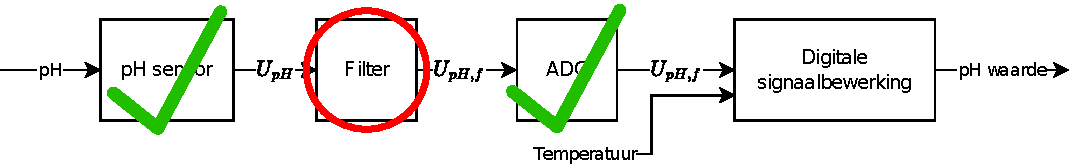
\includegraphics[width=0.95\textwidth]{signaalverwerking_filter.pdf}
    \caption{Het blokschema van de signaalverwerking, met het filter omcirkeld.}
    \label{fig:filterInSchema}
\end{figure}

\begin{figure}[!htbp]
    \centering
    \def\svgwidth{0.4\textwidth}
    \input{img/filterBlok.pdf_tex}
    \caption{Het filterblok.}
    \label{fig:filterBlok}
\end{figure}


\subsubsection{Orde bepalen} \label{sec:DetermineAAorder}
De orde van het filter en de kantelfrequentie bepalen hoeveel demping er op een zekere frequentie plaatsvindt. De demping van een nde orde Butterworth filter op frequentie $f_s$ en met het kantel punt op $f_c$ kan met \cref{eq:dampingOfTheFilter} berekend worden \cite{electronicFilterDesignHandbook}.
\begin{equation} \label{eq:dampingOfTheFilter}
    D_{dB}=10\log\left(1+\left(\frac{f_s}{f_c}\right)^{2n}\right)
\end{equation}

In het geval een Butterworth filter gebruikt wordt om een anti aliasing filter te implementeren moet de maximaal toelaatbare demping voor de hoogste signaal frequentie van interesse worden bepaalt. Daarnaast moet de minimale demping van de stop band worden gespecificeerd. Het is dan mogelijk om met \cref{eq:minOrderOfAAfilter} de minimale orde van het anti aliasing filter te berekenen.
Wanneer er bewust gebruik wordt gemaakt van aliasing moet er een banddoorlaatfilter worden gebruikt. In dit verslag zal hier echter niet op in worden gegaan.

Om te bepalen welke orde een laag/hoog filter nodig heeft is het belangrijk om te weten hoeveel het filter de hoogste signaal frequentie van interesse mag dempen. De hoogste signaal frequentie van interesse wordt gegeven door $f_h$ in Hz en de maximale demping in dB die op deze frequentie mag optreden wordt gegeven door $D_D$. Ook moet bekend zijn wat de minimale demping in dB gegeven door $D_D$ op de hoogst toelaatbare frequentie moet zijn, deze frequentie wordt gegeven door $f_D$.
\begin{equation} \label{eq:minOrderOfAAfilter}
    n=\left\lceil\frac{1}{2}\ln\left(\frac{10^{D_D/10}-1}{10^{D_h/10}-1}\right)\frac{1}{\ln\left(\frac{f_D}{f_h}\right)}\right\rceil
    \tagaddtext{[order]}
\end{equation}

Omdat de minimale orde van het filter berekend kan worden, kan uitgerekend worden wat de minimale en maximale kantel frequentie van het filter is door \cref{eq:boundriesFc} te gebruiken. Bij het implementeren van het filter kan de kantelfrequentie hoger dan wel lager worden vanwege spreiding in de component waardes. Doordat de afwijking van componenten zowel omhoog als omlaag kunnen gaan is het niet mogelijk om te voorspellen of de afwijking van de kantelfrequentie voornamelijk omhoog dan wel omlaag zal gaan. Om hier rekening mee te houden is het aan te raden om de kantelfrequentie halverwege deze twee limieten te kiezen. Deze frequentie is uit te rekenen met \cref{eq:calcCutoffFreqFilter}. Door gebruik te maken van \cref{eq:calcAllowedCutofFreqDeviation} is het mogelijk om uit te rekenen hoeveel de kantelfrequentie mag afwijken van de berekende kantelfrequentie met \cref{eq:calcCutoffFreqFilter}.
\begin{equation}\label{eq:boundriesFc}
    \frac{f_h}{\left(10^{D_h/10}-1\right)^{2n}}\leqslant f_c\leqslant\frac{f_D}{\left(10^{D_D/10}-1\right)^{2n}}
    \tagaddtext{[\si{\hertz}]}
\end{equation}
\begin{equation}\label{eq:calcCutoffFreqFilter}
    f_c=\frac{1}{2}\left(\frac{f_h}{\left(10^{D_h/10}-1\right)^{\frac{1}{2n}}}+\frac{f_D}{\left(10^{D_D/10}-1\right)^{\frac{1}{2n}}}\right)
    \tagaddtext{[\si{\hertz}]}
\end{equation}
\begin{equation}\label{eq:calcAllowedCutofFreqDeviation}
    \epsilon_{f_c}=\frac{1}{2}\left(\frac{f_D}{\left(10^{D_D/10}-1\right)^{\frac{1}{2n}}}-\frac{f_h}{\left(10^{D_h/10}-1\right)^{\frac{1}{2n}}}\right)
    \tagaddtext{[\si{\hertz}]}
\end{equation}

\begin{figure}[!htbp]
    \centering
    \input{plots/filterorder.tex}
    \caption{Eigenschappen van de kantelfrequentie ten gevolge van de orde van het filter.}
    \label{fig:fcEigenschappenTengevolgeVanN}
\end{figure}
% kantelfrequentie + limiet n -> infty
Zoals eerder aangegeven kan met \cref{eq:calcCutoffFreqFilter} de benodigde kantelfrequentie voor een filter worden berekend. \Cref{eq:calcCutoffFreqFilter} houdt er geen rekening mee of de filter orde hoog genoeg is en berekend enkel het gemiddelde van de benodigde kantelfrequentie van $f_h$ met $D_h$ en $f_D$ met $D_D$. In \cref{fig:fcEigenschappenTengevolgeVanN}\footnote{Er is voor deze grafiek gebruik gemaakt van de filter specificaties van het te ontwerpen filter in dit project.} is te zien dat \cref{eq:calcCutoffFreqFilter} naar een waarde toegaat wanneer n naar oneindig gaat. \Cref{eq:limietCutoffFreqNtoInfty} toont het resultaat van $\lim_{n\rightarrow\infty}f_c\left(n\right)$. Dit laat zien dat wanneer er een filter wordt gebruikt met een orde die naar oneindig gaat de kantelfrequentie het gemiddelde wordt van $f_h$ en $f_D$.
\begin{equation}\label{eq:limietCutoffFreqNtoInfty}
    f_{c,n\infty}=\frac{f_h+f_D}{2}
\end{equation}
De maximale afwijking van de kantelfrequentie van een filter is ook afhankelijk van de orde van het filter. \Cref{eq:maxErrorFc} kan worden gevonden, door: $\lim_{n\rightarrow\infty}\epsilon_{f_c}\left(n\right)$ op te lossen. Een andere manier op \cref{eq:maxErrorFc} te beredeneren is dat met een oneindig hoge filter orde de dempingseis oneindig snel kan worden behaald. Dit beteknt dat de kantelfrequentie niet voor/op $f_h$ maar wel voor/op $f_D$ moet uitkomen. \Cref{eq:maxErrorFc} kan worden gebruikt om te controleren of het mogelijk is om aan de filter eisen van de kantelfrequentie te voldoen.
\begin{equation}\label{eq:maxErrorFc}
    \epsilon_{f_c,n\infty}=\frac{f_D-f_h}{2}
\end{equation}
% afwijking + limiet n -> infty
% bla bla

% procentuele afwijking
% negatief
% limiet n -> infty


\subsubsection{Eerste orde}
Wanneer er een eerste orde passief laagdoorlaatfilter wordt gebruikt is het mogelijk om een aantal eigenschappen verder uit te werken.
De schakeling van een eerste orde passief laagdoorlaatfilter is te zien in \cref{fig:filterCircuit}. De kantelfrequentie van een eerste orde passief laagdoorlaatfilter afhankelijk van de $C$ en $R$, volgens \cref{eq:cutoffFreq}.
\begin{figure}[ht]
    \centering
    \def\svgwidth{0.3\textwidth}
    \subsection{Filter}
Tussen de ADC en de uitleesschakeling van de sensor zit een filter. Dit filter zorgt ervoor dat alle frequenties buiten de bandbreedte weggefilterd worden. Er is gekozen om hiervoor een eerste orde filter te gebruiken.
De schakeling van dit filter is te zien in \autoref{fig:filterCircuit}. De kantelfrequentie het filter ligt aan de waardes van $C$ en $R$, volgens \autoref{eq:cutoffFreq}.

\subsubsection{Ruis}
De spectrale ruisdichtheid aan de ingang van het filter is te berekenen met \autoref{eq:filterNoiseDensity}.
De spectrale ruisdichtheid aan de uitgang van het filter is hetzelfde als die van de spanningsdeler in \autoref{sec:referenceVoltage}. Deze is te berekenen met \autoref{eq:dividerNoise}.

\begin{figure}[ht]
    \centering
    \def\svgwidth{0.3\textwidth}
    \subsection{Filter}
Tussen de ADC en de uitleesschakeling van de sensor zit een filter. Dit filter zorgt ervoor dat alle frequenties buiten de bandbreedte weggefilterd worden. Er is gekozen om hiervoor een eerste orde filter te gebruiken.
De schakeling van dit filter is te zien in \autoref{fig:filterCircuit}. De kantelfrequentie het filter ligt aan de waardes van $C$ en $R$, volgens \autoref{eq:cutoffFreq}.

\subsubsection{Ruis}
De spectrale ruisdichtheid aan de ingang van het filter is te berekenen met \autoref{eq:filterNoiseDensity}.
De spectrale ruisdichtheid aan de uitgang van het filter is hetzelfde als die van de spanningsdeler in \autoref{sec:referenceVoltage}. Deze is te berekenen met \autoref{eq:dividerNoise}.

\begin{figure}[ht]
    \centering
    \def\svgwidth{0.3\textwidth}
    \subsection{Filter}
Tussen de ADC en de uitleesschakeling van de sensor zit een filter. Dit filter zorgt ervoor dat alle frequenties buiten de bandbreedte weggefilterd worden. Er is gekozen om hiervoor een eerste orde filter te gebruiken.
De schakeling van dit filter is te zien in \autoref{fig:filterCircuit}. De kantelfrequentie het filter ligt aan de waardes van $C$ en $R$, volgens \autoref{eq:cutoffFreq}.

\subsubsection{Ruis}
De spectrale ruisdichtheid aan de ingang van het filter is te berekenen met \autoref{eq:filterNoiseDensity}.
De spectrale ruisdichtheid aan de uitgang van het filter is hetzelfde als die van de spanningsdeler in \autoref{sec:referenceVoltage}. Deze is te berekenen met \autoref{eq:dividerNoise}.

\begin{figure}[ht]
    \centering
    \def\svgwidth{0.3\textwidth}
    \input{img/filter.pdf_tex}
    \caption{Het eerste-orde filter.}
    \label{fig:filterCircuit}
\end{figure}

% TODO: BEPAAL OVERDRACHT

\begin{equation} \label{eq:cutoffFreq}
    2\pi f_c = \omega_c = \frac{1}{RC}
    \tagaddtext{[\si{\radian\per\second}]}
\end{equation}

% \begin{equation} \label{eq:filterTransfer}
%     H(s) = \frac{1}{1+sRC}
% \end{equation}

\begin{equation} \label{eq:filterNoiseDensity}
    S_{u_{in}} = 4kTR
    \tagaddtext{[\si{\volt\squared\per\hertz}]}
\end{equation}

% De signaal-ruis verhouding aan de uitgang van dit filter is te berekenen met \autoref{eq:filterSNR}
% \begin{equation}\label{eq:filterSNR}
%     \mathrm{SNR} = 20\log\left(U_{out,min}\sqrt{\frac{C}{kT}}\right)
%     \tagaddtext{[\si{\decibel}]}
% \end{equation}

\subsubsection{Vermogen}
Het vermogensverbruik van het filter is te berekenen met \autoref{eq:filterPowerLaplace}.
\begin{equation} \label{eq:filterPowerLaplace}
    P = \frac{U_{in,max}^2}{\left|R + \frac{1}{sC}\right|}
    \tagaddtext{[\si{\watt}]}
\end{equation}
Omdat volgens \autoref{eq:cutoffFreq} $R$ te definiëren is in $\omega_c$ en $C$, volgt hieruit \autoref{eq:filterPower}.
\begin{equation} \label{eq:filterPower}
    P = \frac{1}{\sqrt{2}}\omega_cCU_{in,max}^2
    \tagaddtext{[\si{\watt}]}
\end{equation}
Uit deze formule is te zien dat het vermogensverbruik lineair evenredig is met de condensatorwaarde. Om het vermogensverbruik te minimaliseren moet dus een zo klein mogelijk condensatorwaarde gekozen worden. Aangezien de noise-figure van dit filter maximaal 3dB mag zijn, mag dit filter maximaal evenveel spanningsruis genereren als het systeem ervoor. Hieruit volgt \autoref{eq:dividerNoise}, waarmee de minimale condensatorwaarde te berekenen is. Hierbij is $u_{n,in}$ de ruisspanning aan de ingang van het filter.
\begin{equation} \label{eq:filterCapMin}
    C_{min} = \frac{kT}{u_{n,in}^2}
    \tagaddtext{[\si{\farad}]}
\end{equation}
    \caption{Het eerste-orde filter.}
    \label{fig:filterCircuit}
\end{figure}

% TODO: BEPAAL OVERDRACHT

\begin{equation} \label{eq:cutoffFreq}
    2\pi f_c = \omega_c = \frac{1}{RC}
    \tagaddtext{[\si{\radian\per\second}]}
\end{equation}

% \begin{equation} \label{eq:filterTransfer}
%     H(s) = \frac{1}{1+sRC}
% \end{equation}

\begin{equation} \label{eq:filterNoiseDensity}
    S_{u_{in}} = 4kTR
    \tagaddtext{[\si{\volt\squared\per\hertz}]}
\end{equation}

% De signaal-ruis verhouding aan de uitgang van dit filter is te berekenen met \autoref{eq:filterSNR}
% \begin{equation}\label{eq:filterSNR}
%     \mathrm{SNR} = 20\log\left(U_{out,min}\sqrt{\frac{C}{kT}}\right)
%     \tagaddtext{[\si{\decibel}]}
% \end{equation}

\subsubsection{Vermogen}
Het vermogensverbruik van het filter is te berekenen met \autoref{eq:filterPowerLaplace}.
\begin{equation} \label{eq:filterPowerLaplace}
    P = \frac{U_{in,max}^2}{\left|R + \frac{1}{sC}\right|}
    \tagaddtext{[\si{\watt}]}
\end{equation}
Omdat volgens \autoref{eq:cutoffFreq} $R$ te definiëren is in $\omega_c$ en $C$, volgt hieruit \autoref{eq:filterPower}.
\begin{equation} \label{eq:filterPower}
    P = \frac{1}{\sqrt{2}}\omega_cCU_{in,max}^2
    \tagaddtext{[\si{\watt}]}
\end{equation}
Uit deze formule is te zien dat het vermogensverbruik lineair evenredig is met de condensatorwaarde. Om het vermogensverbruik te minimaliseren moet dus een zo klein mogelijk condensatorwaarde gekozen worden. Aangezien de noise-figure van dit filter maximaal 3dB mag zijn, mag dit filter maximaal evenveel spanningsruis genereren als het systeem ervoor. Hieruit volgt \autoref{eq:dividerNoise}, waarmee de minimale condensatorwaarde te berekenen is. Hierbij is $u_{n,in}$ de ruisspanning aan de ingang van het filter.
\begin{equation} \label{eq:filterCapMin}
    C_{min} = \frac{kT}{u_{n,in}^2}
    \tagaddtext{[\si{\farad}]}
\end{equation}
    \caption{Het eerste-orde filter.}
    \label{fig:filterCircuit}
\end{figure}

% TODO: BEPAAL OVERDRACHT

\begin{equation} \label{eq:cutoffFreq}
    2\pi f_c = \omega_c = \frac{1}{RC}
    \tagaddtext{[\si{\radian\per\second}]}
\end{equation}

% \begin{equation} \label{eq:filterTransfer}
%     H(s) = \frac{1}{1+sRC}
% \end{equation}

\begin{equation} \label{eq:filterNoiseDensity}
    S_{u_{in}} = 4kTR
    \tagaddtext{[\si{\volt\squared\per\hertz}]}
\end{equation}

% De signaal-ruis verhouding aan de uitgang van dit filter is te berekenen met \autoref{eq:filterSNR}
% \begin{equation}\label{eq:filterSNR}
%     \mathrm{SNR} = 20\log\left(U_{out,min}\sqrt{\frac{C}{kT}}\right)
%     \tagaddtext{[\si{\decibel}]}
% \end{equation}

\subsubsection{Vermogen}
Het vermogensverbruik van het filter is te berekenen met \autoref{eq:filterPowerLaplace}.
\begin{equation} \label{eq:filterPowerLaplace}
    P = \frac{U_{in,max}^2}{\left|R + \frac{1}{sC}\right|}
    \tagaddtext{[\si{\watt}]}
\end{equation}
Omdat volgens \autoref{eq:cutoffFreq} $R$ te definiëren is in $\omega_c$ en $C$, volgt hieruit \autoref{eq:filterPower}.
\begin{equation} \label{eq:filterPower}
    P = \frac{1}{\sqrt{2}}\omega_cCU_{in,max}^2
    \tagaddtext{[\si{\watt}]}
\end{equation}
Uit deze formule is te zien dat het vermogensverbruik lineair evenredig is met de condensatorwaarde. Om het vermogensverbruik te minimaliseren moet dus een zo klein mogelijk condensatorwaarde gekozen worden. Aangezien de noise-figure van dit filter maximaal 3dB mag zijn, mag dit filter maximaal evenveel spanningsruis genereren als het systeem ervoor. Hieruit volgt \autoref{eq:dividerNoise}, waarmee de minimale condensatorwaarde te berekenen is. Hierbij is $u_{n,in}$ de ruisspanning aan de ingang van het filter.
\begin{equation} \label{eq:filterCapMin}
    C_{min} = \frac{kT}{u_{n,in}^2}
    \tagaddtext{[\si{\farad}]}
\end{equation}
    \caption{Het eerste-orde filter.}
    \label{fig:filterCircuit}
\end{figure}
\begin{equation} \label{eq:cutoffFreq}
    2\pi f_c = \omega_c = \frac{1}{RC}
    \tagaddtext{[\si{\radian\per\second}]}
\end{equation}

\subsubsection{Ruis}
De spectrale ruisdichtheid aan de ingang van het filter is te berekenen met \cref{eq:filterNoiseDensity}.
De spectrale ruisdichtheid aan de uitgang van het filter is hetzelfde als die van de spanningsdeler in \cref{sec:referenceVoltage}. Deze is te berekenen met \cref{eq:dividerNoise}.


% TODO: BEPAAL OVERDRACHT

% \begin{equation} \label{eq:filterTransfer}
%     H(s) = \frac{1}{1+sRC}
% \end{equation}

\begin{equation} \label{eq:filterNoiseDensity}
    S_{u_{in}} = 4kTR
    \tagaddtext{[\si{\volt\squared\per\hertz}]}
\end{equation}

% De signaal-ruis verhouding aan de uitgang van dit filter is te berekenen met \cref{eq:filterSNR}
% \begin{equation}\label{eq:filterSNR}
%     \mathrm{SNR} = 20\log\left(U_{out,min}\sqrt{\frac{C}{kT}}\right)
%     \tagaddtext{[\si{\decibel}]}
% \end{equation}

\subsubsection{Vermogen}
Het vermogensverbruik van het filter is te berekenen met \cref{eq:filterPowerLaplace}.
\begin{equation} \label{eq:filterPowerLaplace}
    P = \frac{U_{in,max}^2}{\left|R + \frac{1}{sC}\right|}
    \tagaddtext{[\si{\watt}]}
\end{equation}
Omdat volgens \cref{eq:cutoffFreq} $R$ te definiëren is in $\omega_c$ en $C$, volgt hieruit \cref{eq:filterPower}.
\begin{equation} \label{eq:filterPower}
    P = \frac{1}{2}\omega_cCU_{in,max}^2
    \tagaddtext{[\si{\watt}]}
\end{equation}
In deze formule is te zien dat het vermogensverbruik lineair evenredig is met de condensatorwaarde. Om het vermogensverbruik te minimaliseren moet dus een zo klein mogelijke condensatorwaarde gekozen worden. Aangezien de noise-figure van dit filter maximaal 3dB mag zijn, mag dit filter maximaal evenveel spanningsruis genereren als het systeem ervoor. Hieruit volgt \cref{eq:filterCapMin}, waarmee de minimale condensatorwaarde te berekenen is. Hierbij is $u_{n,in}$ de RMS ruisspanning aan de ingang van het filter.
\begin{equation} \label{eq:filterCapMin}
    C_{min} = \frac{kT}{u_{n,in}^2\left(10^{NF/10}-1\right)}
    \tagaddtext{[\si{\farad}]}
\end{equation}

\subsubsection{Specificaties}
% In ... is
In de voorgaande paragrafen is in gegaan op hoe specificaties voor discriminatie in het frequentie domain de eigenschappen van een filter kunnen worden berekend. Hieronder staan deze specificaties:
\begin{itemize}
    \item $f_h$, de hoogste signaalfrequentie van interesse
    \item $D_h$, de maximale demping in dB op de hoogste signaalfrequentie van interesse
    \item $f_D$, de frequentie waarop er een minimale demping moet zijn bereikt
    \item $D_D$, de minimale demping in dB op $f_D$
    \item $\overline{u_{n,in}}$, de uitgangsgerefereerde ruis van het voorgaande systeem
    \item $NF$, dit geeft aan hoeveel ruis het filter mag produceren afhankelijk van $\overline{u_{n,in}}$
\end{itemize}

De eisen die aan het filter worden gesteld kunnen gehaald worden uit de systeemspecificaties in combinatie met het systeemdiagram. In \cref{tab:prelimenarySpecsAAfilter} staan de resulterende specificaties voor het anti aliasing laagdoorlaatfilter.
\begin{table}[ht]
    \centering
    \begin{tabular}{c|c|c}
        Specificatie & Waarde & Eenheid \\\hline
        $f_h$ & 10 & $[\si{\hertz}]$\\
        $D_f$ & 3   & $[\mathrm{dB}]$ \\
        $f_d$ &  & $[\si{\hertz}]$ \\
        $D_D$ & 37   & $[\mathrm{dB}]$ \\
        $\overline{u_{n,in}}$ & & $[\si{\volt^2}]$\\
        $NF$ & 3 & $[\mathrm{dB}]$
    \end{tabular}
    \caption{De tot nu toe bekende specificaties voor het anti aliasing laagdoorlaatfilter.}
    \label{tab:prelimenarySpecsAAfilter}
\end{table}

Een aantal specificaties van het filter zijn afhankelijk van de implementatie van het voorgaande en opvolgende systeem. Deze afhankelijkheden zullen dus eerst moeten worden bepaalt in het voorgaande/opvolgende systeem, voordat het filter geïmplementeerd kan worden. Een afhankelijkheid van het voorgaande systeem is, de uitgangsgerefereerde ruis van de ISFET uitleesschakeling.
Een afhankelijkheid van het opvolgende systeem is, $f_d$ die afhankelijk is van de ADC sample frequentie.